\documentclass[twoside]{book}

% Packages required by doxygen
\usepackage{fixltx2e}
\usepackage{calc}
\usepackage{doxygen}
\usepackage[export]{adjustbox} % also loads graphicx
\usepackage{graphicx}
\usepackage[utf8]{inputenc}
\usepackage{makeidx}
\usepackage{multicol}
\usepackage{multirow}
\PassOptionsToPackage{warn}{textcomp}
\usepackage{textcomp}
\usepackage[nointegrals]{wasysym}
\usepackage[table]{xcolor}

% Font selection
\usepackage[T1]{fontenc}
\usepackage[scaled=.90]{helvet}
\usepackage{courier}
\usepackage{amssymb}
\usepackage{sectsty}
\renewcommand{\familydefault}{\sfdefault}
\allsectionsfont{%
  \fontseries{bc}\selectfont%
  \color{darkgray}%
}
\renewcommand{\DoxyLabelFont}{%
  \fontseries{bc}\selectfont%
  \color{darkgray}%
}
\newcommand{\+}{\discretionary{\mbox{\scriptsize$\hookleftarrow$}}{}{}}

% Page & text layout
\usepackage{geometry}
\geometry{%
  a4paper,%
  top=2.5cm,%
  bottom=2.5cm,%
  left=2.5cm,%
  right=2.5cm%
}
\tolerance=750
\hfuzz=15pt
\hbadness=750
\setlength{\emergencystretch}{15pt}
\setlength{\parindent}{0cm}
\setlength{\parskip}{3ex plus 2ex minus 2ex}
\makeatletter
\renewcommand{\paragraph}{%
  \@startsection{paragraph}{4}{0ex}{-1.0ex}{1.0ex}{%
    \normalfont\normalsize\bfseries\SS@parafont%
  }%
}
\renewcommand{\subparagraph}{%
  \@startsection{subparagraph}{5}{0ex}{-1.0ex}{1.0ex}{%
    \normalfont\normalsize\bfseries\SS@subparafont%
  }%
}
\makeatother

% Headers & footers
\usepackage{fancyhdr}
\pagestyle{fancyplain}
\fancyhead[LE]{\fancyplain{}{\bfseries\thepage}}
\fancyhead[CE]{\fancyplain{}{}}
\fancyhead[RE]{\fancyplain{}{\bfseries\leftmark}}
\fancyhead[LO]{\fancyplain{}{\bfseries\rightmark}}
\fancyhead[CO]{\fancyplain{}{}}
\fancyhead[RO]{\fancyplain{}{\bfseries\thepage}}
\fancyfoot[LE]{\fancyplain{}{}}
\fancyfoot[CE]{\fancyplain{}{}}
\fancyfoot[RE]{\fancyplain{}{\bfseries\scriptsize Generated by Doxygen }}
\fancyfoot[LO]{\fancyplain{}{\bfseries\scriptsize Generated by Doxygen }}
\fancyfoot[CO]{\fancyplain{}{}}
\fancyfoot[RO]{\fancyplain{}{}}
\renewcommand{\footrulewidth}{0.4pt}
\renewcommand{\chaptermark}[1]{%
  \markboth{#1}{}%
}
\renewcommand{\sectionmark}[1]{%
  \markright{\thesection\ #1}%
}

% Indices & bibliography
\usepackage{natbib}
\usepackage[titles]{tocloft}
\setcounter{tocdepth}{3}
\setcounter{secnumdepth}{5}
\makeindex

% Hyperlinks (required, but should be loaded last)
\usepackage{ifpdf}
\ifpdf
  \usepackage[pdftex,pagebackref=true]{hyperref}
\else
  \usepackage[ps2pdf,pagebackref=true]{hyperref}
\fi
\hypersetup{%
  colorlinks=true,%
  linkcolor=blue,%
  citecolor=blue,%
  unicode%
}

% Custom commands
\newcommand{\clearemptydoublepage}{%
  \newpage{\pagestyle{empty}\cleardoublepage}%
}

\usepackage{caption}
\captionsetup{labelsep=space,justification=centering,font={bf},singlelinecheck=off,skip=4pt,position=top}

%===== C O N T E N T S =====

\begin{document}

% Titlepage & ToC
\hypersetup{pageanchor=false,
             bookmarksnumbered=true,
             pdfencoding=unicode
            }
\pagenumbering{roman}
\begin{titlepage}
\vspace*{7cm}
\begin{center}%
{\Large exp\+\_\+assignment2 }\\
\vspace*{1cm}
{\large Generated by Doxygen 1.8.11}\\
\end{center}
\end{titlepage}
\clearemptydoublepage
\tableofcontents
\clearemptydoublepage
\pagenumbering{arabic}
\hypersetup{pageanchor=true}

%--- Begin generated contents ---
\chapter{Hierarchical Index}
\section{Class Hierarchy}
This inheritance list is sorted roughly, but not completely, alphabetically\+:\begin{DoxyCompactList}
\item \contentsline{section}{state\+\_\+manager.\+find\+\_\+and\+\_\+follow\+\_\+ball}{\pageref{classstate__manager_1_1find__and__follow__ball}}{}
\item State\begin{DoxyCompactList}
\item \contentsline{section}{state\+\_\+manager.\+M\+I\+R\+O\+\_\+\+Normal}{\pageref{classstate__manager_1_1MIRO__Normal}}{}
\item \contentsline{section}{state\+\_\+manager.\+M\+I\+R\+O\+\_\+\+Play}{\pageref{classstate__manager_1_1MIRO__Play}}{}
\item \contentsline{section}{state\+\_\+manager.\+M\+I\+R\+O\+\_\+\+Sleep}{\pageref{classstate__manager_1_1MIRO__Sleep}}{}
\end{DoxyCompactList}
\end{DoxyCompactList}

\chapter{Class Index}
\section{Class List}
Here are the classes, structs, unions and interfaces with brief descriptions\+:\begin{DoxyCompactList}
\item\contentsline{section}{\hyperlink{classstate__manager_1_1find__and__follow__ball}{state\+\_\+manager.\+find\+\_\+and\+\_\+follow\+\_\+ball} \\*This class is used to detect and follow the green ball in the arena }{\pageref{classstate__manager_1_1find__and__follow__ball}}{}
\item\contentsline{section}{\hyperlink{classstate__manager_1_1MIRO__Normal}{state\+\_\+manager.\+M\+I\+R\+O\+\_\+\+Normal} \\*Normal state of the smach machine }{\pageref{classstate__manager_1_1MIRO__Normal}}{}
\item\contentsline{section}{\hyperlink{classstate__manager_1_1MIRO__Play}{state\+\_\+manager.\+M\+I\+R\+O\+\_\+\+Play} \\*Play state of the smach machine }{\pageref{classstate__manager_1_1MIRO__Play}}{}
\item\contentsline{section}{\hyperlink{classstate__manager_1_1MIRO__Sleep}{state\+\_\+manager.\+M\+I\+R\+O\+\_\+\+Sleep} \\*Sleep state of the smach machine }{\pageref{classstate__manager_1_1MIRO__Sleep}}{}
\end{DoxyCompactList}

\chapter{File Index}
\section{File List}
Here is a list of all documented files with brief descriptions\+:\begin{DoxyCompactList}
\item\contentsline{section}{scripts/{\bfseries go\+\_\+to\+\_\+point\+\_\+ball.\+py} }{\pageref{go__to__point__ball_8py}}{}
\item\contentsline{section}{scripts/{\bfseries go\+\_\+to\+\_\+point\+\_\+robot.\+py} }{\pageref{go__to__point__robot_8py}}{}
\item\contentsline{section}{scripts/\hyperlink{human__commands_8py}{human\+\_\+commands.\+py} \\*This node implements an actionlib client to move the ball-\/ }{\pageref{human__commands_8py}}{}
\item\contentsline{section}{scripts/\hyperlink{state__manager_8py}{state\+\_\+manager.\+py} \\*This node implements a smach state machine to simulate a dog that can sleep, play and wander around }{\pageref{state__manager_8py}}{}
\end{DoxyCompactList}

\chapter{Class Documentation}
\hypertarget{classstate__manager_1_1find__and__follow__ball}{}\section{state\+\_\+manager.\+find\+\_\+and\+\_\+follow\+\_\+ball Class Reference}
\label{classstate__manager_1_1find__and__follow__ball}\index{state\+\_\+manager.\+find\+\_\+and\+\_\+follow\+\_\+ball@{state\+\_\+manager.\+find\+\_\+and\+\_\+follow\+\_\+ball}}


This class is used to detect and follow the green ball in the arena.  


\subsection*{Public Member Functions}
\begin{DoxyCompactItemize}
\item 
def \hyperlink{classstate__manager_1_1find__and__follow__ball_a6469e8486bd8e40cd87f77d93add522a}{\+\_\+\+\_\+init\+\_\+\+\_\+} (self)
\begin{DoxyCompactList}\small\item\em It initializes a publisher to the image, one to the robot velocity and one to the camera motor. \end{DoxyCompactList}\item 
def \hyperlink{classstate__manager_1_1find__and__follow__ball_ab8dc079ef8ce39c9679ed9e5428b4e8c}{callback} (self, ros\+\_\+data)
\begin{DoxyCompactList}\small\item\em This function is the callback function of the subscription to the camera image. \end{DoxyCompactList}\end{DoxyCompactItemize}
\subsection*{Public Attributes}
\begin{DoxyCompactItemize}
\item 
{\bfseries image\+\_\+pub}\hypertarget{classstate__manager_1_1find__and__follow__ball_aff00cf94531440a3c05f404e3a7157ed}{}\label{classstate__manager_1_1find__and__follow__ball_aff00cf94531440a3c05f404e3a7157ed}

\item 
{\bfseries vel\+\_\+pub}\hypertarget{classstate__manager_1_1find__and__follow__ball_acfadf373311857d7df4a48ee0bba0271}{}\label{classstate__manager_1_1find__and__follow__ball_acfadf373311857d7df4a48ee0bba0271}

\item 
{\bfseries camera\+\_\+pub}\hypertarget{classstate__manager_1_1find__and__follow__ball_a6d047759897ca99cbb11fd39f8861ab9}{}\label{classstate__manager_1_1find__and__follow__ball_a6d047759897ca99cbb11fd39f8861ab9}

\item 
{\bfseries subscriber}\hypertarget{classstate__manager_1_1find__and__follow__ball_aa9a2ffdc682841e5efdaf5a6b80ec0eb}{}\label{classstate__manager_1_1find__and__follow__ball_aa9a2ffdc682841e5efdaf5a6b80ec0eb}

\end{DoxyCompactItemize}


\subsection{Detailed Description}
This class is used to detect and follow the green ball in the arena. 



Definition at line 123 of file state\+\_\+manager.\+py.



\subsection{Constructor \& Destructor Documentation}
\index{state\+\_\+manager\+::find\+\_\+and\+\_\+follow\+\_\+ball@{state\+\_\+manager\+::find\+\_\+and\+\_\+follow\+\_\+ball}!\+\_\+\+\_\+init\+\_\+\+\_\+@{\+\_\+\+\_\+init\+\_\+\+\_\+}}
\index{\+\_\+\+\_\+init\+\_\+\+\_\+@{\+\_\+\+\_\+init\+\_\+\+\_\+}!state\+\_\+manager\+::find\+\_\+and\+\_\+follow\+\_\+ball@{state\+\_\+manager\+::find\+\_\+and\+\_\+follow\+\_\+ball}}
\subsubsection[{\texorpdfstring{\+\_\+\+\_\+init\+\_\+\+\_\+(self)}{__init__(self)}}]{\setlength{\rightskip}{0pt plus 5cm}def state\+\_\+manager.\+find\+\_\+and\+\_\+follow\+\_\+ball.\+\_\+\+\_\+init\+\_\+\+\_\+ (
\begin{DoxyParamCaption}
\item[{}]{self}
\end{DoxyParamCaption}
)}\hypertarget{classstate__manager_1_1find__and__follow__ball_a6469e8486bd8e40cd87f77d93add522a}{}\label{classstate__manager_1_1find__and__follow__ball_a6469e8486bd8e40cd87f77d93add522a}


It initializes a publisher to the image, one to the robot velocity and one to the camera motor. 

It subscribes to the camera image \begin{DoxyVerb}Initialize ros publisher, ros subscriber\end{DoxyVerb}
 

Definition at line 127 of file state\+\_\+manager.\+py.


\begin{DoxyCode}
127     \textcolor{keyword}{def }\hyperlink{classstate__manager_1_1find__and__follow__ball_a6469e8486bd8e40cd87f77d93add522a}{\_\_init\_\_}(self):
128         \textcolor{stringliteral}{'''Initialize ros publisher, ros subscriber'''}
129 
130         \textcolor{comment}{# Init publishers}
131         self.\hyperlink{classstate__manager_1_1find__and__follow__ball_aff00cf94531440a3c05f404e3a7157ed}{image\_pub} = rospy.Publisher(\textcolor{stringliteral}{"/output/image\_raw/compressed"},
132                                          CompressedImage, queue\_size=1)
133         self.\hyperlink{classstate__manager_1_1find__and__follow__ball_acfadf373311857d7df4a48ee0bba0271}{vel\_pub} = rospy.Publisher(\textcolor{stringliteral}{"/robot/cmd\_vel"},
134                                        Twist, queue\_size=1)
135         self.\hyperlink{classstate__manager_1_1find__and__follow__ball_a6d047759897ca99cbb11fd39f8861ab9}{camera\_pub} = rospy.Publisher(
136             \textcolor{stringliteral}{"/robot/joint\_position\_controller/command"}, Float64, queue\_size=1)
137 
138         \textcolor{comment}{# Subscribed Topic}
139         self.\hyperlink{classstate__manager_1_1find__and__follow__ball_aa9a2ffdc682841e5efdaf5a6b80ec0eb}{subscriber} = rospy.Subscriber(\textcolor{stringliteral}{"/robot/camera1/image\_raw/compressed"},
140                                            CompressedImage, self.\hyperlink{classstate__manager_1_1find__and__follow__ball_ab8dc079ef8ce39c9679ed9e5428b4e8c}{callback},  queue\_size=1)
141 
\end{DoxyCode}


\subsection{Member Function Documentation}
\index{state\+\_\+manager\+::find\+\_\+and\+\_\+follow\+\_\+ball@{state\+\_\+manager\+::find\+\_\+and\+\_\+follow\+\_\+ball}!callback@{callback}}
\index{callback@{callback}!state\+\_\+manager\+::find\+\_\+and\+\_\+follow\+\_\+ball@{state\+\_\+manager\+::find\+\_\+and\+\_\+follow\+\_\+ball}}
\subsubsection[{\texorpdfstring{callback(self, ros\+\_\+data)}{callback(self, ros_data)}}]{\setlength{\rightskip}{0pt plus 5cm}def state\+\_\+manager.\+find\+\_\+and\+\_\+follow\+\_\+ball.\+callback (
\begin{DoxyParamCaption}
\item[{}]{self, }
\item[{}]{ros\+\_\+data}
\end{DoxyParamCaption}
)}\hypertarget{classstate__manager_1_1find__and__follow__ball_ab8dc079ef8ce39c9679ed9e5428b4e8c}{}\label{classstate__manager_1_1find__and__follow__ball_ab8dc079ef8ce39c9679ed9e5428b4e8c}


This function is the callback function of the subscription to the camera image. 

It looks for a green contour in the image, plots a circle around it and makes the robot approach it. When the robot has the object at a specified distance, it stops, turns its head twice and again looks for the object. If the robot doesn\textquotesingle{}t see the ball for 10 iterations in a row, it sets the ros parameter counter to 10 and then waits for it to be zero again. 

Definition at line 147 of file state\+\_\+manager.\+py.


\begin{DoxyCode}
147     \textcolor{keyword}{def }\hyperlink{classstate__manager_1_1find__and__follow__ball_ab8dc079ef8ce39c9679ed9e5428b4e8c}{callback}(self, ros\_data):
148         \textcolor{keyword}{global} counter
149         \textcolor{keyword}{global} vel\_camera
150         \textcolor{keyword}{global} MAX\_COUNTER
151 
152         \textcolor{comment}{# Read counter ros parameter: proceed only if it's not max}
153         counter = rospy.get\_param(\textcolor{stringliteral}{'counter'})
154         \textcolor{keywordflow}{while} counter == MAX\_COUNTER:
155             time.sleep(1)
156 
157         \textcolor{keywordflow}{if} VERBOSE:
158             print(\textcolor{stringliteral}{'received image of type: "%s"'} % ros\_data.format)
159 
160         \textcolor{comment}{# Convert to cv2}
161         np\_arr = np.fromstring(ros\_data.data, np.uint8)
162         image\_np = cv2.imdecode(np\_arr, cv2.IMREAD\_COLOR)  \textcolor{comment}{# OpenCV >= 3.0:}
163 
164         \textcolor{comment}{# Color limits}
165         greenLower = (50, 50, 20)
166         greenUpper = (70, 255, 255)
167 
168         \textcolor{comment}{# Create masks}
169         blurred = cv2.GaussianBlur(image\_np, (11, 11), 0)
170         hsv = cv2.cvtColor(blurred, cv2.COLOR\_BGR2HSV)
171         mask = cv2.inRange(hsv, greenLower, greenUpper)
172         mask = cv2.erode(mask, \textcolor{keywordtype}{None}, iterations=2)
173         mask = cv2.dilate(mask, \textcolor{keywordtype}{None}, iterations=2)
174 
175         \textcolor{comment}{# Find contour}
176         cnts = cv2.findContours(mask.copy(), cv2.RETR\_EXTERNAL,
177                                 cv2.CHAIN\_APPROX\_SIMPLE)
178         cnts = imutils.grab\_contours(cnts)
179         center = \textcolor{keywordtype}{None}
180 
181         \textcolor{comment}{# Only proceed if at least one contour was found}
182         \textcolor{keywordflow}{if} len(cnts) > 0:
183 
184             \textcolor{comment}{# Find the largest contour in the mask, then use it to compute the minimum enclosing circle and
       centroid}
185             c = max(cnts, key=cv2.contourArea)
186             ((x, y), radius) = cv2.minEnclosingCircle(c)
187             M = cv2.moments(c)
188             center = (int(M[\textcolor{stringliteral}{"m10"}] / M[\textcolor{stringliteral}{"m00"}]), int(M[\textcolor{stringliteral}{"m01"}] / M[\textcolor{stringliteral}{"m00"}]))
189 
190             \textcolor{comment}{# Only proceed if the radius meets a minimum size}
191             \textcolor{keywordflow}{if} radius > 10:
192 
193                 \textcolor{comment}{# Draw the circle and centroid on the frame, then update the list of tracked points}
194                 cv2.circle(image\_np, (int(x), int(y)), int(radius),
195                            (0, 255, 255), 2)
196                 cv2.circle(image\_np, center, 5, (0, 0, 255), -1)
197                 vel\_Play = Twist()
198 
199                 \textcolor{comment}{# Publish robot vel}
200                 vel\_Play.angular.z = -0.002*(center[0]-400)
201                 vel\_Play.linear.x = -0.01*(radius-100)
202                 self.vel\_pub.publish(vel\_Play)
203 
204                 \textcolor{comment}{# When robot has arrived: turn head}
205                 \textcolor{keywordflow}{if} vel\_Play.linear.x <= 0.05 \textcolor{keywordflow}{and} vel\_Play.angular.z <= 0.05:
206 
207                     \textcolor{comment}{# Stop robot completely}
208                     vel\_Play.angular.z = 0
209                     vel\_Play.linear.x = 0
210                     self.vel\_pub.publish(vel\_Play)
211 
212                     \textcolor{comment}{# Rotate camera}
213                     rospy.set\_param(\textcolor{stringliteral}{'rotate\_camera'}, 1)
214 
215             \textcolor{comment}{# Go near ball}
216             \textcolor{keywordflow}{else}:
217                 vel\_Play = Twist()
218                 vel\_Play.linear.x = 0.5
219                 self.vel\_pub.publish(vel\_Play)
220 
221         \textcolor{comment}{# Look for ball by turning on the spot}
222         \textcolor{keywordflow}{else}:
223             vel\_Play = Twist()
224             vel\_Play.angular.z = 0.5
225             self.vel\_pub.publish(vel\_Play)
226 
227             \textcolor{comment}{# Increase counter of iterations without seeing the ball}
228             counter = counter+1
229             rospy.set\_param(\textcolor{stringliteral}{'counter'}, counter)
230             time.sleep(1)
231             rospy.loginfo(\textcolor{stringliteral}{'counter incremented'})
232 
233             \textcolor{comment}{# If counter is max: stop}
234             \textcolor{keywordflow}{if} counter == MAX\_COUNTER:
235                 vel\_Play.angular.z = 0
236                 self.vel\_pub.publish(vel\_Play)
237                 self.subscriber.unregister()  \textcolor{comment}{# JUST ADDED}
238 
239         \textcolor{comment}{# Show camera image}
240         cv2.imshow(\textcolor{stringliteral}{'window'}, image\_np)
241         cv2.waitKey(2)
242 
\end{DoxyCode}


The documentation for this class was generated from the following file\+:\begin{DoxyCompactItemize}
\item 
scripts/\hyperlink{state__manager_8py}{state\+\_\+manager.\+py}\end{DoxyCompactItemize}

\hypertarget{classstate__manager_1_1MIRO__Normal}{}\section{state\+\_\+manager.\+M\+I\+R\+O\+\_\+\+Normal Class Reference}
\label{classstate__manager_1_1MIRO__Normal}\index{state\+\_\+manager.\+M\+I\+R\+O\+\_\+\+Normal@{state\+\_\+manager.\+M\+I\+R\+O\+\_\+\+Normal}}


Normal state of the smach machine.  




Inheritance diagram for state\+\_\+manager.\+M\+I\+R\+O\+\_\+\+Normal\+:\nopagebreak
\begin{figure}[H]
\begin{center}
\leavevmode
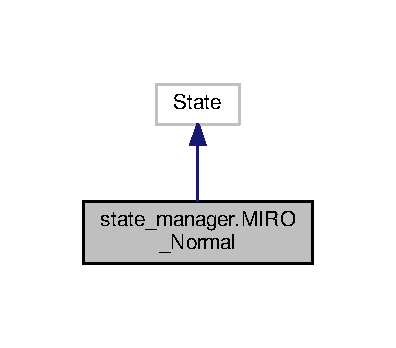
\includegraphics[width=190pt]{classstate__manager_1_1MIRO__Normal__inherit__graph}
\end{center}
\end{figure}


Collaboration diagram for state\+\_\+manager.\+M\+I\+R\+O\+\_\+\+Normal\+:\nopagebreak
\begin{figure}[H]
\begin{center}
\leavevmode
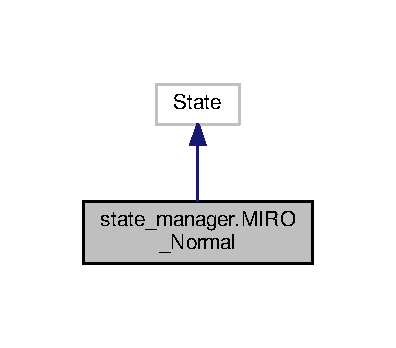
\includegraphics[width=190pt]{classstate__manager_1_1MIRO__Normal__coll__graph}
\end{center}
\end{figure}
\subsection*{Public Member Functions}
\begin{DoxyCompactItemize}
\item 
def \hyperlink{classstate__manager_1_1MIRO__Normal_a36a3ee79119b52beeebd6ee8c04d9501}{\+\_\+\+\_\+init\+\_\+\+\_\+} (self)
\begin{DoxyCompactList}\small\item\em Init function for smach machine normal state. \end{DoxyCompactList}\item 
def \hyperlink{classstate__manager_1_1MIRO__Normal_a4133da39ee6ec170623fc1d457b0729a}{execute} (self, userdata)
\begin{DoxyCompactList}\small\item\em Smach machine state normal actions\+: In a loop\+: Calls \hyperlink{state__manager_8py_ae0155422a2f60744ea3acf5181c7c75a}{move\+\_\+dog()} function to go to a random position, then subscribes to the camera image. \end{DoxyCompactList}\end{DoxyCompactItemize}


\subsection{Detailed Description}
Normal state of the smach machine. 



Definition at line 302 of file state\+\_\+manager.\+py.



\subsection{Constructor \& Destructor Documentation}
\index{state\+\_\+manager\+::\+M\+I\+R\+O\+\_\+\+Normal@{state\+\_\+manager\+::\+M\+I\+R\+O\+\_\+\+Normal}!\+\_\+\+\_\+init\+\_\+\+\_\+@{\+\_\+\+\_\+init\+\_\+\+\_\+}}
\index{\+\_\+\+\_\+init\+\_\+\+\_\+@{\+\_\+\+\_\+init\+\_\+\+\_\+}!state\+\_\+manager\+::\+M\+I\+R\+O\+\_\+\+Normal@{state\+\_\+manager\+::\+M\+I\+R\+O\+\_\+\+Normal}}
\subsubsection[{\texorpdfstring{\+\_\+\+\_\+init\+\_\+\+\_\+(self)}{__init__(self)}}]{\setlength{\rightskip}{0pt plus 5cm}def state\+\_\+manager.\+M\+I\+R\+O\+\_\+\+Normal.\+\_\+\+\_\+init\+\_\+\+\_\+ (
\begin{DoxyParamCaption}
\item[{}]{self}
\end{DoxyParamCaption}
)}\hypertarget{classstate__manager_1_1MIRO__Normal_a36a3ee79119b52beeebd6ee8c04d9501}{}\label{classstate__manager_1_1MIRO__Normal_a36a3ee79119b52beeebd6ee8c04d9501}


Init function for smach machine normal state. 



Definition at line 305 of file state\+\_\+manager.\+py.


\begin{DoxyCode}
305     \textcolor{keyword}{def }\hyperlink{classstate__manager_1_1MIRO__Normal_a36a3ee79119b52beeebd6ee8c04d9501}{\_\_init\_\_}(self):
306 
307         smach.State.\_\_init\_\_(self,
308                              outcomes=[\textcolor{stringliteral}{'sleep\_command'}, \textcolor{stringliteral}{'play\_command'}])
309 
\end{DoxyCode}


\subsection{Member Function Documentation}
\index{state\+\_\+manager\+::\+M\+I\+R\+O\+\_\+\+Normal@{state\+\_\+manager\+::\+M\+I\+R\+O\+\_\+\+Normal}!execute@{execute}}
\index{execute@{execute}!state\+\_\+manager\+::\+M\+I\+R\+O\+\_\+\+Normal@{state\+\_\+manager\+::\+M\+I\+R\+O\+\_\+\+Normal}}
\subsubsection[{\texorpdfstring{execute(self, userdata)}{execute(self, userdata)}}]{\setlength{\rightskip}{0pt plus 5cm}def state\+\_\+manager.\+M\+I\+R\+O\+\_\+\+Normal.\+execute (
\begin{DoxyParamCaption}
\item[{}]{self, }
\item[{}]{userdata}
\end{DoxyParamCaption}
)}\hypertarget{classstate__manager_1_1MIRO__Normal_a4133da39ee6ec170623fc1d457b0729a}{}\label{classstate__manager_1_1MIRO__Normal_a4133da39ee6ec170623fc1d457b0729a}


Smach machine state normal actions\+: In a loop\+: Calls \hyperlink{state__manager_8py_ae0155422a2f60744ea3acf5181c7c75a}{move\+\_\+dog()} function to go to a random position, then subscribes to the camera image. 

It reads the ball ros parameter\+: if it\textquotesingle{}s set to 2 it waits. If it\textquotesingle{}s set to 0, it moves the robot to another random position. If it\textquotesingle{}s set to 1 it switches to play state. At the end of the loop\+: it switches to sleep state. \begin{DoxyReturn}{Returns}
c\+: command to switch between states. 
\end{DoxyReturn}


Definition at line 317 of file state\+\_\+manager.\+py.


\begin{DoxyCode}
317     \textcolor{keyword}{def }\hyperlink{classstate__manager_1_1MIRO__Normal_a4133da39ee6ec170623fc1d457b0729a}{execute}(self, userdata):
318 
319         \textcolor{keyword}{global} subscriberNORM, LOOPS
320 
321         \textcolor{keywordflow}{for} i \textcolor{keywordflow}{in} range(0, LOOPS):
322 
323             \textcolor{comment}{# Go rand (then set rand)}
324             time.sleep(3)
325             rospy.loginfo(\textcolor{stringliteral}{'normal: going rand'})
326             \textcolor{comment}{# ([random.randrange(0, 9),random.randrange(0, 9), 0])}
327             move\_dog([-5, 5, 0])
328 
329             \textcolor{comment}{# Look for ball}
330             time.sleep(3)
331             rospy.loginfo(\textcolor{stringliteral}{'normal: looking for ball'})
332             subscriberNORM = rospy.Subscriber(\textcolor{stringliteral}{"camera1/image\_raw/compressed"},
333                                               CompressedImage, find\_ball,  queue\_size=1)
334 
335             \textcolor{keywordflow}{while} rospy.get\_param(\textcolor{stringliteral}{'ball'}) == 2:
336                 time.sleep(1)
337 
338             ball = rospy.get\_param(\textcolor{stringliteral}{'ball'})
339             rospy.set\_param(\textcolor{stringliteral}{'ball'}, 2)
340 
341             \textcolor{comment}{# Case 0: no ball --> continue in normal state}
342             \textcolor{keywordflow}{if} ball == 0:
343                 rospy.loginfo(
344                     \textcolor{stringliteral}{'normal: i see no ball, i will continue doing my things'})
345 
346             \textcolor{comment}{# Case 1: ball --> go in play state}
347             \textcolor{keywordflow}{elif} ball == 1:
348                 rospy.loginfo(
349                     \textcolor{stringliteral}{'normal: i do see ball, i will chase it: set play'})
350 
351                 c = \textcolor{stringliteral}{'play\_command'}
352                 \textcolor{keywordflow}{return} c
353 
354             \textcolor{comment}{# Case err: ball wasn't set yet}
355             \textcolor{keywordflow}{else}:
356                 rospy.loginfo(\textcolor{stringliteral}{'normal: ball was not set yet'})
357                 time.sleep(3)
358 
359         c = \textcolor{stringliteral}{'sleep\_command'}
360         \textcolor{keywordflow}{return} c
361 
362 
\end{DoxyCode}


The documentation for this class was generated from the following file\+:\begin{DoxyCompactItemize}
\item 
scripts/\hyperlink{state__manager_8py}{state\+\_\+manager.\+py}\end{DoxyCompactItemize}

\hypertarget{classstate__manager_1_1MIRO__Play}{}\section{state\+\_\+manager.\+M\+I\+R\+O\+\_\+\+Play Class Reference}
\label{classstate__manager_1_1MIRO__Play}\index{state\+\_\+manager.\+M\+I\+R\+O\+\_\+\+Play@{state\+\_\+manager.\+M\+I\+R\+O\+\_\+\+Play}}


Play state of the smach machine.  




Inheritance diagram for state\+\_\+manager.\+M\+I\+R\+O\+\_\+\+Play\+:\nopagebreak
\begin{figure}[H]
\begin{center}
\leavevmode
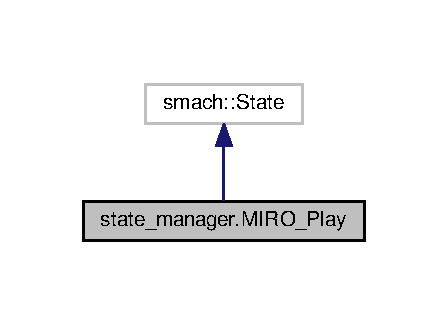
\includegraphics[width=215pt]{classstate__manager_1_1MIRO__Play__inherit__graph}
\end{center}
\end{figure}


Collaboration diagram for state\+\_\+manager.\+M\+I\+R\+O\+\_\+\+Play\+:\nopagebreak
\begin{figure}[H]
\begin{center}
\leavevmode
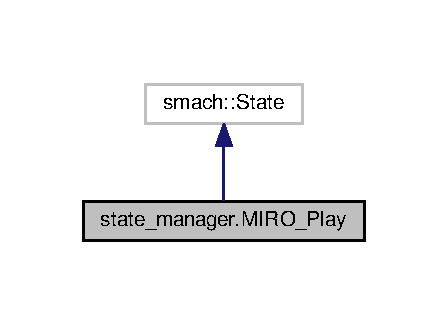
\includegraphics[width=215pt]{classstate__manager_1_1MIRO__Play__coll__graph}
\end{center}
\end{figure}
\subsection*{Public Member Functions}
\begin{DoxyCompactItemize}
\item 
def \hyperlink{classstate__manager_1_1MIRO__Play_a863ae1958460cf6bf33faaba597fc5a2}{\+\_\+\+\_\+init\+\_\+\+\_\+} (self)
\begin{DoxyCompactList}\small\item\em Init function for smach machine play state. \end{DoxyCompactList}\item 
def \hyperlink{classstate__manager_1_1MIRO__Play_a781db4be4fcbb313c46097a8fdf06275}{execute} (self, userdata)
\begin{DoxyCompactList}\small\item\em Smach machine state play actions\+: find and follow the ball. \end{DoxyCompactList}\end{DoxyCompactItemize}
\subsection*{Public Attributes}
\begin{DoxyCompactItemize}
\item 
{\bfseries camera\+\_\+pub}\hypertarget{classstate__manager_1_1MIRO__Play_a72c307cf462ab1c9e0844c84df600078}{}\label{classstate__manager_1_1MIRO__Play_a72c307cf462ab1c9e0844c84df600078}

\end{DoxyCompactItemize}


\subsection{Detailed Description}
Play state of the smach machine. 



Definition at line 366 of file state\+\_\+manager.\+py.



\subsection{Constructor \& Destructor Documentation}
\index{state\+\_\+manager\+::\+M\+I\+R\+O\+\_\+\+Play@{state\+\_\+manager\+::\+M\+I\+R\+O\+\_\+\+Play}!\+\_\+\+\_\+init\+\_\+\+\_\+@{\+\_\+\+\_\+init\+\_\+\+\_\+}}
\index{\+\_\+\+\_\+init\+\_\+\+\_\+@{\+\_\+\+\_\+init\+\_\+\+\_\+}!state\+\_\+manager\+::\+M\+I\+R\+O\+\_\+\+Play@{state\+\_\+manager\+::\+M\+I\+R\+O\+\_\+\+Play}}
\subsubsection[{\texorpdfstring{\+\_\+\+\_\+init\+\_\+\+\_\+(self)}{__init__(self)}}]{\setlength{\rightskip}{0pt plus 5cm}def state\+\_\+manager.\+M\+I\+R\+O\+\_\+\+Play.\+\_\+\+\_\+init\+\_\+\+\_\+ (
\begin{DoxyParamCaption}
\item[{}]{self}
\end{DoxyParamCaption}
)}\hypertarget{classstate__manager_1_1MIRO__Play_a863ae1958460cf6bf33faaba597fc5a2}{}\label{classstate__manager_1_1MIRO__Play_a863ae1958460cf6bf33faaba597fc5a2}


Init function for smach machine play state. 



Definition at line 369 of file state\+\_\+manager.\+py.


\begin{DoxyCode}
369     \textcolor{keyword}{def }\hyperlink{classstate__manager_1_1MIRO__Play_a863ae1958460cf6bf33faaba597fc5a2}{\_\_init\_\_}(self):
370 
371         smach.State.\_\_init\_\_(self,
372                              outcomes=[\textcolor{stringliteral}{'normal\_command'}])
373 
374         self.\hyperlink{classstate__manager_1_1MIRO__Play_a72c307cf462ab1c9e0844c84df600078}{camera\_pub} = rospy.Publisher(\textcolor{stringliteral}{"/robot/joint\_position\_controller/command"},
375                                           Float64, queue\_size=1)
376 
\end{DoxyCode}


\subsection{Member Function Documentation}
\index{state\+\_\+manager\+::\+M\+I\+R\+O\+\_\+\+Play@{state\+\_\+manager\+::\+M\+I\+R\+O\+\_\+\+Play}!execute@{execute}}
\index{execute@{execute}!state\+\_\+manager\+::\+M\+I\+R\+O\+\_\+\+Play@{state\+\_\+manager\+::\+M\+I\+R\+O\+\_\+\+Play}}
\subsubsection[{\texorpdfstring{execute(self, userdata)}{execute(self, userdata)}}]{\setlength{\rightskip}{0pt plus 5cm}def state\+\_\+manager.\+M\+I\+R\+O\+\_\+\+Play.\+execute (
\begin{DoxyParamCaption}
\item[{}]{self, }
\item[{}]{userdata}
\end{DoxyParamCaption}
)}\hypertarget{classstate__manager_1_1MIRO__Play_a781db4be4fcbb313c46097a8fdf06275}{}\label{classstate__manager_1_1MIRO__Play_a781db4be4fcbb313c46097a8fdf06275}


Smach machine state play actions\+: find and follow the ball. 

If robot reaches the ball and stops\+: rotate camera. If robot can not see ball for a while (counter=M\+A\+X\+\_\+\+C\+O\+U\+N\+T\+ER)\+: switch to normal state. \begin{DoxyReturn}{Returns}
c\+: command to switch between states. 
\end{DoxyReturn}


Definition at line 381 of file state\+\_\+manager.\+py.


\begin{DoxyCode}
381     \textcolor{keyword}{def }\hyperlink{classstate__manager_1_1MIRO__Play_a781db4be4fcbb313c46097a8fdf06275}{execute}(self, userdata):
382 
383         \textcolor{keyword}{global} subscriberPLAY
384         \textcolor{keyword}{global} MAX\_COUNTER
385 
386         time.sleep(3)
387         rospy.loginfo(\textcolor{stringliteral}{'play: chase ball'})
388 
389         \textcolor{comment}{# Find and follow green ball}
390         ic = \hyperlink{classstate__manager_1_1find__and__follow__ball}{find\_and\_follow\_ball}()
391         rotated = 0
392 
393         \textcolor{keywordflow}{while} rospy.get\_param(\textcolor{stringliteral}{'counter'}) < MAX\_COUNTER:
394             \textcolor{stringliteral}{'''}
395 \textcolor{stringliteral}{            time.sleep(3)}
396 \textcolor{stringliteral}{            if rotated == 1:}
397 \textcolor{stringliteral}{                time.sleep(10)}
398 \textcolor{stringliteral}{}
399 \textcolor{stringliteral}{            rotated = 0}
400 \textcolor{stringliteral}{            '''}
401 
402             \textcolor{keywordflow}{if} rospy.get\_param(\textcolor{stringliteral}{'rotate\_camera'}) == 1:
403 
404                 rospy.loginfo(\textcolor{stringliteral}{'rotating camera'})
405                 vel\_camera.data = 0
406 
407                 \textcolor{comment}{# Turn head left}
408                 \textcolor{keywordflow}{while} vel\_camera.data < 0.5:
409                     vel\_camera.data = vel\_camera.data + 0.1
410                     self.camera\_pub.publish(vel\_camera)
411                     time.sleep(1)
412 
413                 \textcolor{comment}{# Turn head to center}
414                 \textcolor{keywordflow}{while} vel\_camera.data > 0.01:
415                     vel\_camera.data = vel\_camera.data - 0.1
416                     self.camera\_pub.publish(vel\_camera)
417                     time.sleep(1)
418 
419                 \textcolor{comment}{# Turn head right}
420                 \textcolor{keywordflow}{while} vel\_camera.data > 0.5:
421                     vel\_camera.data = vel\_camera.data - 0.1
422                     self.camera\_pub.publish(vel\_camera)
423                     time.sleep(1)
424 
425                 \textcolor{comment}{# Turn head to center}
426                 \textcolor{keywordflow}{while} vel\_camera.data < 0.01:
427                     vel\_camera.data = vel\_camera.data + 0.1
428                     self.camera\_pub.publish(vel\_camera)
429                     time.sleep(1)
430 
431                 \textcolor{comment}{# Rotation finished}
432                 rospy.set\_param(\textcolor{stringliteral}{'rotate\_camera'}, 0)
433 
434                 \textcolor{comment}{# Wait until dog can't see the ball no more, and switch to normal state}
435                 rospy.set\_param(\textcolor{stringliteral}{'counter'}, 0)  \textcolor{comment}{# JUST MODIFIED}
436 
437         rospy.loginfo(\textcolor{stringliteral}{'back to normal, havent seen ball for a while'})
438         c = \textcolor{stringliteral}{'normal\_command'}
439         \textcolor{keywordflow}{return} c
440 
441 
\end{DoxyCode}


The documentation for this class was generated from the following file\+:\begin{DoxyCompactItemize}
\item 
scripts/\hyperlink{state__manager_8py}{state\+\_\+manager.\+py}\end{DoxyCompactItemize}

\hypertarget{classstate__manager_1_1MIRO__Sleep}{}\section{state\+\_\+manager.\+M\+I\+R\+O\+\_\+\+Sleep Class Reference}
\label{classstate__manager_1_1MIRO__Sleep}\index{state\+\_\+manager.\+M\+I\+R\+O\+\_\+\+Sleep@{state\+\_\+manager.\+M\+I\+R\+O\+\_\+\+Sleep}}


Sleep state of the smach machine.  




Inheritance diagram for state\+\_\+manager.\+M\+I\+R\+O\+\_\+\+Sleep\+:\nopagebreak
\begin{figure}[H]
\begin{center}
\leavevmode
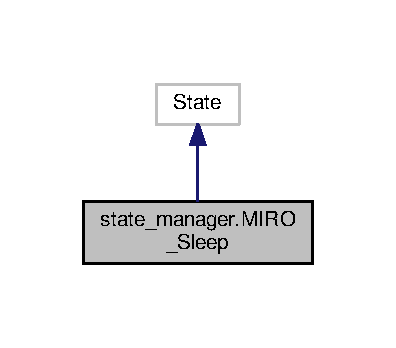
\includegraphics[width=190pt]{classstate__manager_1_1MIRO__Sleep__inherit__graph}
\end{center}
\end{figure}


Collaboration diagram for state\+\_\+manager.\+M\+I\+R\+O\+\_\+\+Sleep\+:\nopagebreak
\begin{figure}[H]
\begin{center}
\leavevmode
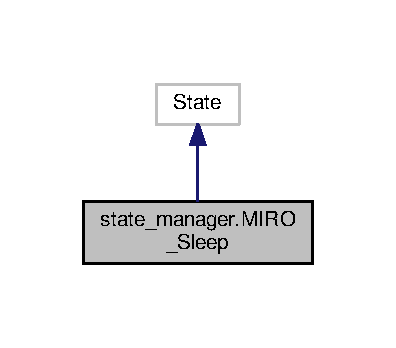
\includegraphics[width=190pt]{classstate__manager_1_1MIRO__Sleep__coll__graph}
\end{center}
\end{figure}
\subsection*{Public Member Functions}
\begin{DoxyCompactItemize}
\item 
def \hyperlink{classstate__manager_1_1MIRO__Sleep_a1e0695b96023b2c827bd28d9b0c11bfb}{\+\_\+\+\_\+init\+\_\+\+\_\+} (self)
\begin{DoxyCompactList}\small\item\em Init function for smach machine sleep state. \end{DoxyCompactList}\item 
def \hyperlink{classstate__manager_1_1MIRO__Sleep_acda704c667aad40c16f10d7c705b1b2e}{execute} (self, userdata)
\begin{DoxyCompactList}\small\item\em Smach machine state sleep actions\+: Calls dog() function to move towards the kennel, waits some seconds and exits state. \end{DoxyCompactList}\end{DoxyCompactItemize}


\subsection{Detailed Description}
Sleep state of the smach machine. 



Definition at line 276 of file state\+\_\+manager.\+py.



\subsection{Constructor \& Destructor Documentation}
\index{state\+\_\+manager\+::\+M\+I\+R\+O\+\_\+\+Sleep@{state\+\_\+manager\+::\+M\+I\+R\+O\+\_\+\+Sleep}!\+\_\+\+\_\+init\+\_\+\+\_\+@{\+\_\+\+\_\+init\+\_\+\+\_\+}}
\index{\+\_\+\+\_\+init\+\_\+\+\_\+@{\+\_\+\+\_\+init\+\_\+\+\_\+}!state\+\_\+manager\+::\+M\+I\+R\+O\+\_\+\+Sleep@{state\+\_\+manager\+::\+M\+I\+R\+O\+\_\+\+Sleep}}
\subsubsection[{\texorpdfstring{\+\_\+\+\_\+init\+\_\+\+\_\+(self)}{__init__(self)}}]{\setlength{\rightskip}{0pt plus 5cm}def state\+\_\+manager.\+M\+I\+R\+O\+\_\+\+Sleep.\+\_\+\+\_\+init\+\_\+\+\_\+ (
\begin{DoxyParamCaption}
\item[{}]{self}
\end{DoxyParamCaption}
)}\hypertarget{classstate__manager_1_1MIRO__Sleep_a1e0695b96023b2c827bd28d9b0c11bfb}{}\label{classstate__manager_1_1MIRO__Sleep_a1e0695b96023b2c827bd28d9b0c11bfb}


Init function for smach machine sleep state. 



Definition at line 279 of file state\+\_\+manager.\+py.


\begin{DoxyCode}
279     \textcolor{keyword}{def }\hyperlink{classstate__manager_1_1MIRO__Sleep_a1e0695b96023b2c827bd28d9b0c11bfb}{\_\_init\_\_}(self):
280 
281         smach.State.\_\_init\_\_(self,
282                              outcomes=[\textcolor{stringliteral}{'normal\_command'}])
283 
\end{DoxyCode}


\subsection{Member Function Documentation}
\index{state\+\_\+manager\+::\+M\+I\+R\+O\+\_\+\+Sleep@{state\+\_\+manager\+::\+M\+I\+R\+O\+\_\+\+Sleep}!execute@{execute}}
\index{execute@{execute}!state\+\_\+manager\+::\+M\+I\+R\+O\+\_\+\+Sleep@{state\+\_\+manager\+::\+M\+I\+R\+O\+\_\+\+Sleep}}
\subsubsection[{\texorpdfstring{execute(self, userdata)}{execute(self, userdata)}}]{\setlength{\rightskip}{0pt plus 5cm}def state\+\_\+manager.\+M\+I\+R\+O\+\_\+\+Sleep.\+execute (
\begin{DoxyParamCaption}
\item[{}]{self, }
\item[{}]{userdata}
\end{DoxyParamCaption}
)}\hypertarget{classstate__manager_1_1MIRO__Sleep_acda704c667aad40c16f10d7c705b1b2e}{}\label{classstate__manager_1_1MIRO__Sleep_acda704c667aad40c16f10d7c705b1b2e}


Smach machine state sleep actions\+: Calls dog() function to move towards the kennel, waits some seconds and exits state. 

\begin{DoxyReturn}{Returns}
c\+: command to switch between states. 
\end{DoxyReturn}


Definition at line 287 of file state\+\_\+manager.\+py.


\begin{DoxyCode}
287     \textcolor{keyword}{def }\hyperlink{classstate__manager_1_1MIRO__Sleep_acda704c667aad40c16f10d7c705b1b2e}{execute}(self, userdata):
288 
289         \textcolor{comment}{# Go home and sleep}
290         time.sleep(3)
291         rospy.loginfo(\textcolor{stringliteral}{'sleep: go home'})
292         move\_dog([0, 0, 0])
293         time.sleep(5)
294 
295         \textcolor{comment}{# Change state}
296         c = \textcolor{stringliteral}{'normal\_command'}
297         \textcolor{keywordflow}{return} c
298 
\end{DoxyCode}


The documentation for this class was generated from the following file\+:\begin{DoxyCompactItemize}
\item 
scripts/\hyperlink{state__manager_8py}{state\+\_\+manager.\+py}\end{DoxyCompactItemize}

\chapter{File Documentation}
\hypertarget{human__commands_8py}{}\section{scripts/human\+\_\+commands.py File Reference}
\label{human__commands_8py}\index{scripts/human\+\_\+commands.\+py@{scripts/human\+\_\+commands.\+py}}


This node implements an actionlib client to move the ball-\/.  


\subsection*{Functions}
\begin{DoxyCompactItemize}
\item 
def \hyperlink{human__commands_8py_a7897d0129a9e28f290c26ca1f37e9aed}{human\+\_\+commands.\+human\+\_\+client} ()
\begin{DoxyCompactList}\small\item\em This function implements a client for the ball motion server. \end{DoxyCompactList}\item 
def \hyperlink{human__commands_8py_a8b958e887d5a5424271cf6a9cc1fc067}{human\+\_\+commands.\+main} ()\hypertarget{human__commands_8py_a8b958e887d5a5424271cf6a9cc1fc067}{}\label{human__commands_8py_a8b958e887d5a5424271cf6a9cc1fc067}

\begin{DoxyCompactList}\small\item\em Ros node that calls the client for the ball motion server. \end{DoxyCompactList}\end{DoxyCompactItemize}


\subsection{Detailed Description}
This node implements an actionlib client to move the ball-\/. 



\subsection{Function Documentation}
\index{human\+\_\+commands.\+py@{human\+\_\+commands.\+py}!human\+\_\+client@{human\+\_\+client}}
\index{human\+\_\+client@{human\+\_\+client}!human\+\_\+commands.\+py@{human\+\_\+commands.\+py}}
\subsubsection[{\texorpdfstring{human\+\_\+client()}{human_client()}}]{\setlength{\rightskip}{0pt plus 5cm}def human\+\_\+commands.\+human\+\_\+client (
\begin{DoxyParamCaption}
{}
\end{DoxyParamCaption}
)}\hypertarget{human__commands_8py_file_a7897d0129a9e28f290c26ca1f37e9aed}{}\label{human__commands_8py_file_a7897d0129a9e28f290c26ca1f37e9aed}


This function implements a client for the ball motion server. 



Definition at line 24 of file human\+\_\+commands.\+py.


\begin{DoxyCode}
24 \textcolor{keyword}{def }human\_client():
25 
26     client = actionlib.SimpleActionClient(
27         \textcolor{stringliteral}{'/reaching\_goal'}, exp\_assignment2.msg.PlanningAction)
28 
29     \textcolor{comment}{# Waits until the action server has started up and started}
30     \textcolor{comment}{# listening for goals.}
31     client.wait\_for\_server()
32 
33     \textcolor{comment}{# Creates a goal to send to the action server.}
34     goal = exp\_assignment2.msg.PlanningGoal()
35     \textcolor{stringliteral}{'''}
36 \textcolor{stringliteral}{    rospy.loginfo('print x')}
37 \textcolor{stringliteral}{    in1 = int(input())}
38 \textcolor{stringliteral}{    rospy.loginfo('print y')}
39 \textcolor{stringliteral}{    in2 = int(input())}
40 \textcolor{stringliteral}{    rospy.loginfo('print z')}
41 \textcolor{stringliteral}{    in3 = int(input())}
42 \textcolor{stringliteral}{    '''}
43     goal.target\_pose.pose.position.x = random.randrange(0, 9)
44     goal.target\_pose.pose.position.y = random.randrange(0, 9)
45     goal.target\_pose.pose.position.z = random.choice([0, 1, 10])
46 
47     \textcolor{comment}{# Sends the goal to the action server.}
48     client.send\_goal(goal)
49 
50     \textcolor{comment}{# Waits for the server to finish performing the action.}
51     client.wait\_for\_result()
52 
53     \textcolor{keywordflow}{return} client.get\_result()
54 
\end{DoxyCode}

\hypertarget{state__manager_8py}{}\section{scripts/state\+\_\+manager.py File Reference}
\label{state__manager_8py}\index{scripts/state\+\_\+manager.\+py@{scripts/state\+\_\+manager.\+py}}


This node implements a smach state machine to simulate a dog that can sleep, play and wander around.  


\subsection*{Classes}
\begin{DoxyCompactItemize}
\item 
class \hyperlink{classstate__manager_1_1find__and__follow__ball}{state\+\_\+manager.\+find\+\_\+and\+\_\+follow\+\_\+ball}
\begin{DoxyCompactList}\small\item\em This class is used to detect and follow the green ball in the arena. \end{DoxyCompactList}\item 
class \hyperlink{classstate__manager_1_1MIRO__Sleep}{state\+\_\+manager.\+M\+I\+R\+O\+\_\+\+Sleep}
\begin{DoxyCompactList}\small\item\em Sleep state of the smach machine. \end{DoxyCompactList}\item 
class \hyperlink{classstate__manager_1_1MIRO__Normal}{state\+\_\+manager.\+M\+I\+R\+O\+\_\+\+Normal}
\begin{DoxyCompactList}\small\item\em Normal state of the smach machine. \end{DoxyCompactList}\item 
class \hyperlink{classstate__manager_1_1MIRO__Play}{state\+\_\+manager.\+M\+I\+R\+O\+\_\+\+Play}
\begin{DoxyCompactList}\small\item\em Play state of the smach machine. \end{DoxyCompactList}\end{DoxyCompactItemize}
\subsection*{Functions}
\begin{DoxyCompactItemize}
\item 
def \hyperlink{state__manager_8py_a7d93967d1043bce896aa79f6cc86705c}{state\+\_\+manager.\+find\+\_\+ball} (ros\+\_\+data)
\begin{DoxyCompactList}\small\item\em This function is the callback for the normal state. \end{DoxyCompactList}\item 
def \hyperlink{state__manager_8py_ae0155422a2f60744ea3acf5181c7c75a}{state\+\_\+manager.\+move\+\_\+dog} (target)
\begin{DoxyCompactList}\small\item\em This function is a client for the robot motion server. \end{DoxyCompactList}\item 
def \hyperlink{state__manager_8py_a8663809bc92b964a1202b8888447a326}{state\+\_\+manager.\+main} ()
\begin{DoxyCompactList}\small\item\em Ros node that implements a state machine with three states\+: sleep, play, normal. \end{DoxyCompactList}\end{DoxyCompactItemize}
\subsection*{Variables}
\begin{DoxyCompactItemize}
\item 
bool {\bfseries state\+\_\+manager.\+V\+E\+R\+B\+O\+SE} = False\hypertarget{state__manager_8py_a5a249e9a671c8d36b4b06d0dcdc781cd}{}\label{state__manager_8py_a5a249e9a671c8d36b4b06d0dcdc781cd}

\item 
int {\bfseries state\+\_\+manager.\+L\+O\+O\+PS} = 10\hypertarget{state__manager_8py_afae998fce8866b30be88b687c8614b28}{}\label{state__manager_8py_afae998fce8866b30be88b687c8614b28}

\item 
{\bfseries state\+\_\+manager.\+vel\+\_\+camera} = Float64()\hypertarget{state__manager_8py_a3ae273110e1343ff46f3849c1eb032ec}{}\label{state__manager_8py_a3ae273110e1343ff46f3849c1eb032ec}

\item 
{\bfseries state\+\_\+manager.\+vel\+\_\+\+Norm} = Twist()\hypertarget{state__manager_8py_a0db004eae20055ab41211069e714a2a3}{}\label{state__manager_8py_a0db004eae20055ab41211069e714a2a3}

\item 
int {\bfseries state\+\_\+manager.\+M\+A\+X\+\_\+\+C\+O\+U\+N\+T\+ER} = 25\hypertarget{state__manager_8py_a79442c99330b551fecab75402ef950a2}{}\label{state__manager_8py_a79442c99330b551fecab75402ef950a2}

\item 
int {\bfseries state\+\_\+manager.\+S\+E\+A\+R\+C\+H\+\_\+\+F\+O\+R\+\_\+\+B\+A\+LL} = 15\hypertarget{state__manager_8py_a465127cd3ad4da94ec0432a4b512e9ed}{}\label{state__manager_8py_a465127cd3ad4da94ec0432a4b512e9ed}

\item 
{\bfseries state\+\_\+manager.\+vel\+\_\+pub} = rospy.\+Publisher(\char`\"{}/roboy/cmd\+\_\+vel\char`\"{}, Twist, queue\+\_\+size=1)\hypertarget{state__manager_8py_affa389297adfafddfa44cde69dfd3c2d}{}\label{state__manager_8py_affa389297adfafddfa44cde69dfd3c2d}

\end{DoxyCompactItemize}


\subsection{Detailed Description}
This node implements a smach state machine to simulate a dog that can sleep, play and wander around. 



\subsection{Function Documentation}
\index{state\+\_\+manager.\+py@{state\+\_\+manager.\+py}!find\+\_\+ball@{find\+\_\+ball}}
\index{find\+\_\+ball@{find\+\_\+ball}!state\+\_\+manager.\+py@{state\+\_\+manager.\+py}}
\subsubsection[{\texorpdfstring{find\+\_\+ball(ros\+\_\+data)}{find_ball(ros_data)}}]{\setlength{\rightskip}{0pt plus 5cm}def state\+\_\+manager.\+find\+\_\+ball (
\begin{DoxyParamCaption}
\item[{}]{ros\+\_\+data}
\end{DoxyParamCaption}
)}\hypertarget{state__manager_8py_file_a7d93967d1043bce896aa79f6cc86705c}{}\label{state__manager_8py_file_a7d93967d1043bce896aa79f6cc86705c}


This function is the callback for the normal state. 

It checks if the ball is visible from the camera. If it is\+: it sets the ros parameter ball=1. If it isn\textquotesingle{}t\+: it sets the ros parameter ball=0. 

Definition at line 52 of file state\+\_\+manager.\+py.


\begin{DoxyCode}
52 \textcolor{keyword}{def }find\_ball(ros\_data):
53 
54     \textcolor{keyword}{global} subscriberNORM, vel\_Norm, SEARCH\_FOR\_BALL
55 
56     time.sleep(1)
57 
58     \textcolor{comment}{# Init velocity}
59     vel\_Norm.linear.x = 0
60     vel\_Norm.linear.y = 0
61     vel\_Norm.linear.z = 0
62     vel\_Norm.angular.x = 0
63     vel\_Norm.angular.y = 0
64     vel\_Norm.angular.z = 0
65 
66     \textcolor{comment}{# rospy.loginfo('entered img NORM fnct')}
67 
68     \textcolor{comment}{# Convert to cv2}
69     np\_arr = np.fromstring(ros\_data.data, np.uint8)
70     image\_np = cv2.imdecode(np\_arr, cv2.IMREAD\_COLOR)
71 
72     \textcolor{comment}{# Color limits}
73     greenLower = (50, 50, 20)
74     greenUpper = (70, 255, 255)
75 
76     \textcolor{comment}{# Create masks}
77     blurred = cv2.GaussianBlur(image\_np, (11, 11), 0)
78     hsv = cv2.cvtColor(blurred, cv2.COLOR\_BGR2HSV)
79     mask = cv2.inRange(hsv, greenLower, greenUpper)
80     mask = cv2.erode(mask, \textcolor{keywordtype}{None}, iterations=2)
81     mask = cv2.dilate(mask, \textcolor{keywordtype}{None}, iterations=2)
82 
83     \textcolor{comment}{# Find contour}
84     cnts = cv2.findContours(mask.copy(), cv2.RETR\_EXTERNAL,
85                             cv2.CHAIN\_APPROX\_SIMPLE)
86     cnts = imutils.grab\_contours(cnts)
87     center = \textcolor{keywordtype}{None}
88 
89     \textcolor{comment}{# Only proceed if at least one contour was found}
90     \textcolor{keywordflow}{if} len(cnts) > 0:
91         rospy.loginfo(\textcolor{stringliteral}{'img NORM fnct: ball'})
92         \textcolor{comment}{# Ball was found}
93         rospy.set\_param(\textcolor{stringliteral}{'ball'}, 1)
94         time.sleep(1)
95         subscriberNORM.unregister()
96 
97     \textcolor{keywordflow}{else}:
98         \textcolor{comment}{# Search again in loop}
99         \textcolor{keywordflow}{for} i \textcolor{keywordflow}{in} range(0, SEARCH\_FOR\_BALL):
100             vel\_Norm.angular.z = 0.2
101             vel\_pub.publish(vel\_Norm)
102             time.sleep(1)
103             cnts = cv2.findContours(mask.copy(), cv2.RETR\_EXTERNAL,
104                                     cv2.CHAIN\_APPROX\_SIMPLE)
105             cnts = imutils.grab\_contours(cnts)
106             center = \textcolor{keywordtype}{None}
107 
108             \textcolor{keywordflow}{if} len(cnts) > 0:
109                 rospy.loginfo(\textcolor{stringliteral}{'img NORM fnct: ball after turning'})
110                 \textcolor{comment}{# Ball was found}
111                 rospy.set\_param(\textcolor{stringliteral}{'ball'}, 1)
112                 time.sleep(1)
113                 subscriberNORM.unregister()
114 
115         rospy.loginfo(\textcolor{stringliteral}{'img NORM fnct: no ball'})
116         \textcolor{comment}{# Ball was not found}
117         rospy.set\_param(\textcolor{stringliteral}{'ball'}, 0)
118         time.sleep(1)
119         subscriberNORM.unregister()
120 
121 
\end{DoxyCode}
\index{state\+\_\+manager.\+py@{state\+\_\+manager.\+py}!main@{main}}
\index{main@{main}!state\+\_\+manager.\+py@{state\+\_\+manager.\+py}}
\subsubsection[{\texorpdfstring{main()}{main()}}]{\setlength{\rightskip}{0pt plus 5cm}def state\+\_\+manager.\+main (
\begin{DoxyParamCaption}
{}
\end{DoxyParamCaption}
)}\hypertarget{state__manager_8py_file_a8663809bc92b964a1202b8888447a326}{}\label{state__manager_8py_file_a8663809bc92b964a1202b8888447a326}


Ros node that implements a state machine with three states\+: sleep, play, normal. 

It also initializes the ball and counter parameters. 

Definition at line 446 of file state\+\_\+manager.\+py.


\begin{DoxyCode}
446 \textcolor{keyword}{def }main():
447 
448     rospy.init\_node(\textcolor{stringliteral}{'state\_manager'})
449 
450     \textcolor{comment}{# Init ball ros param to 2 and counter ros param to 0.}
451     rospy.set\_param(\textcolor{stringliteral}{'ball'}, 2)
452     rospy.set\_param(\textcolor{stringliteral}{'counter'}, 0)
453     rospy.set\_param(\textcolor{stringliteral}{'rotate\_camera'}, 0)
454 
455     time.sleep(3)
456 
457     \textcolor{comment}{# Create a SMACH state machine}
458     sm = smach.StateMachine(outcomes=[\textcolor{stringliteral}{'container\_interface'}])
459 
460     with sm:
461         \textcolor{comment}{# Add states to the container}
462         smach.StateMachine.add(\textcolor{stringliteral}{'SLEEP'}, MIRO\_Sleep(),
463                                transitions=\{\textcolor{stringliteral}{'normal\_command'}: \textcolor{stringliteral}{'NORMAL'}\})
464         smach.StateMachine.add(\textcolor{stringliteral}{'NORMAL'}, MIRO\_Normal(),
465                                transitions=\{\textcolor{stringliteral}{'sleep\_command'}: \textcolor{stringliteral}{'SLEEP'},
466                                             \textcolor{stringliteral}{'play\_command'}: \textcolor{stringliteral}{'PLAY'}\})
467         smach.StateMachine.add(\textcolor{stringliteral}{'PLAY'}, MIRO\_Play(),
468                                transitions=\{\textcolor{stringliteral}{'normal\_command'}: \textcolor{stringliteral}{'NORMAL'}\})
469 
470     \textcolor{comment}{# Create and start the introspection server for visualization}
471     sis = smach\_ros.IntrospectionServer(\textcolor{stringliteral}{'server\_name'}, sm, \textcolor{stringliteral}{'/SM\_ROOT'})
472     sis.start()
473 
474     \textcolor{comment}{# Execute the state machine}
475     outcome = sm.execute()
476 
477     \textcolor{comment}{# Wait for ctrl-c to stop the application}
478     rospy.spin()
479     cv2.destroyAllWindows()
480     sis.stop()
481 
482 
\end{DoxyCode}
\index{state\+\_\+manager.\+py@{state\+\_\+manager.\+py}!move\+\_\+dog@{move\+\_\+dog}}
\index{move\+\_\+dog@{move\+\_\+dog}!state\+\_\+manager.\+py@{state\+\_\+manager.\+py}}
\subsubsection[{\texorpdfstring{move\+\_\+dog(target)}{move_dog(target)}}]{\setlength{\rightskip}{0pt plus 5cm}def state\+\_\+manager.\+move\+\_\+dog (
\begin{DoxyParamCaption}
\item[{}]{target}
\end{DoxyParamCaption}
)}\hypertarget{state__manager_8py_file_ae0155422a2f60744ea3acf5181c7c75a}{}\label{state__manager_8py_file_ae0155422a2f60744ea3acf5181c7c75a}


This function is a client for the robot motion server. 

It sends the desired position. 

Definition at line 246 of file state\+\_\+manager.\+py.


\begin{DoxyCode}
246 \textcolor{keyword}{def }move\_dog(target):
247 
248     time.sleep(3)
249 
250     client = actionlib.SimpleActionClient(
251         \textcolor{stringliteral}{'/robot\_reaching\_goal'}, exp\_assignment2.msg.PlanningAction)
252 
253     client.wait\_for\_server()
254 
255     rospy.loginfo(\textcolor{stringliteral}{'Going to %d %d %d'}, target[0], target[1], target[2])
256 
257     \textcolor{comment}{# Creates a goal to send to the action server.}
258     goal = exp\_assignment2.msg.PlanningGoal()
259     goal.target\_pose.pose.position.x = target[0]
260     goal.target\_pose.pose.position.y = target[1]
261     goal.target\_pose.pose.position.z = target[2]
262 
263     \textcolor{comment}{# Sends the goal to the action server.}
264     client.send\_goal(goal)
265 
266     \textcolor{comment}{# Waits for the server to finish performing the action.}
267     client.wait\_for\_result()
268 
269     rospy.loginfo(\textcolor{stringliteral}{'arrived, exiting dog fnct'})
270 
271     \textcolor{keywordflow}{return} client.get\_result()
272 
\end{DoxyCode}

%--- End generated contents ---

% Index
\backmatter
\newpage
\phantomsection
\clearemptydoublepage
\addcontentsline{toc}{chapter}{Index}
\printindex

\end{document}
